% Slides for 2025-02-03
% To create a slide, use the following:
% \begin{frame}{TITLE}
%     BODY
% \end{frame}

% To create a slide with a bullet list, use the following:
% \begin{frame}{TITLE}
%     \begin{itemize}
%         \item ITEM 1
%         \item ITEM 2
%     \end{itemize}    
% \end{frame}

% To create a slide with numbered list, use the following:
% \begin{frame}{TITLE}
%     \begin{enumerate}
%         \item ITEM 1
%         \item ITEM 2
%     \end{enumerate}
% \end{frame}

% To create a slide with a graphic:
% 1. Add the graphic to this folder (named picture.png)
% 2. Use the following:
\begin{frame}{FishSense Mobile}
    \centering
    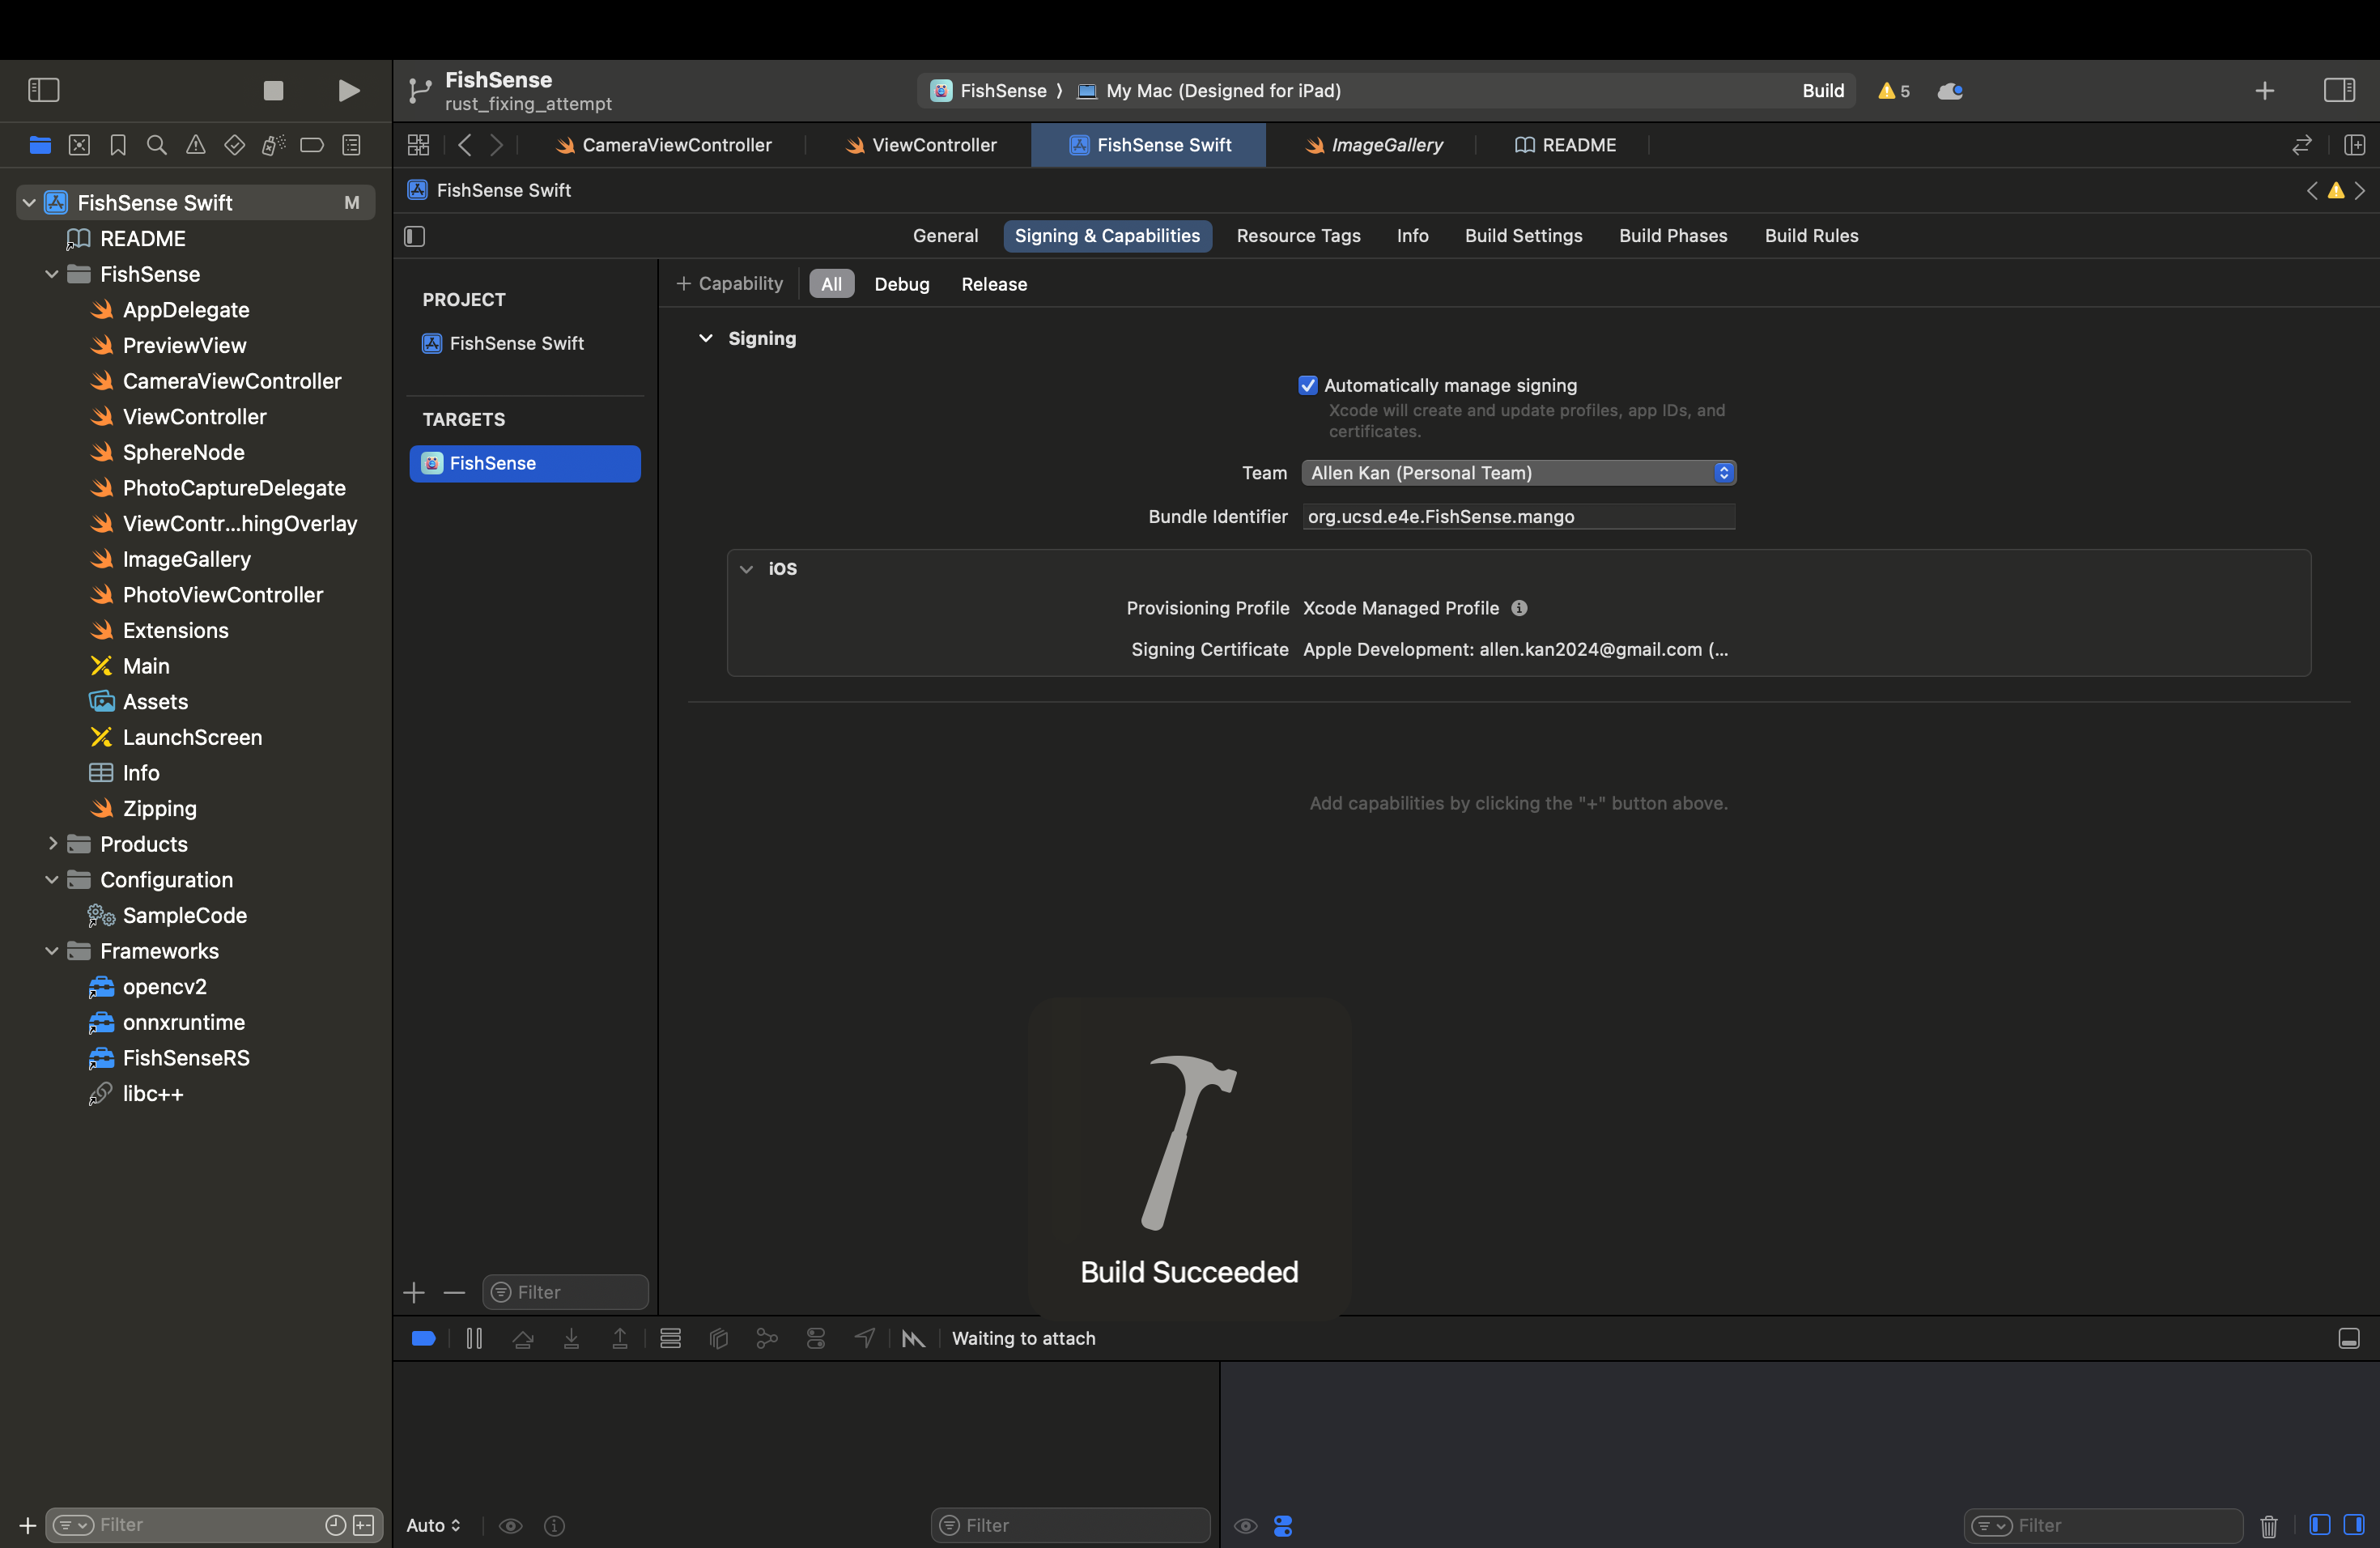
\includegraphics[height=0.75\textheight,width=0.75\textwidth,keepaspectratio]{images/fishsense_enduser/fsmobileBuildSuccess.png}
    \begin{itemize}
        \item Adjusted package dependencies
        \item Newer Rust channel
    \end{itemize}
\end{frame}

\begin{frame}{FishSense Web App: Front-End} 
    \centering
    \begin{minipage}{0.2\textwidth}
        \centering
        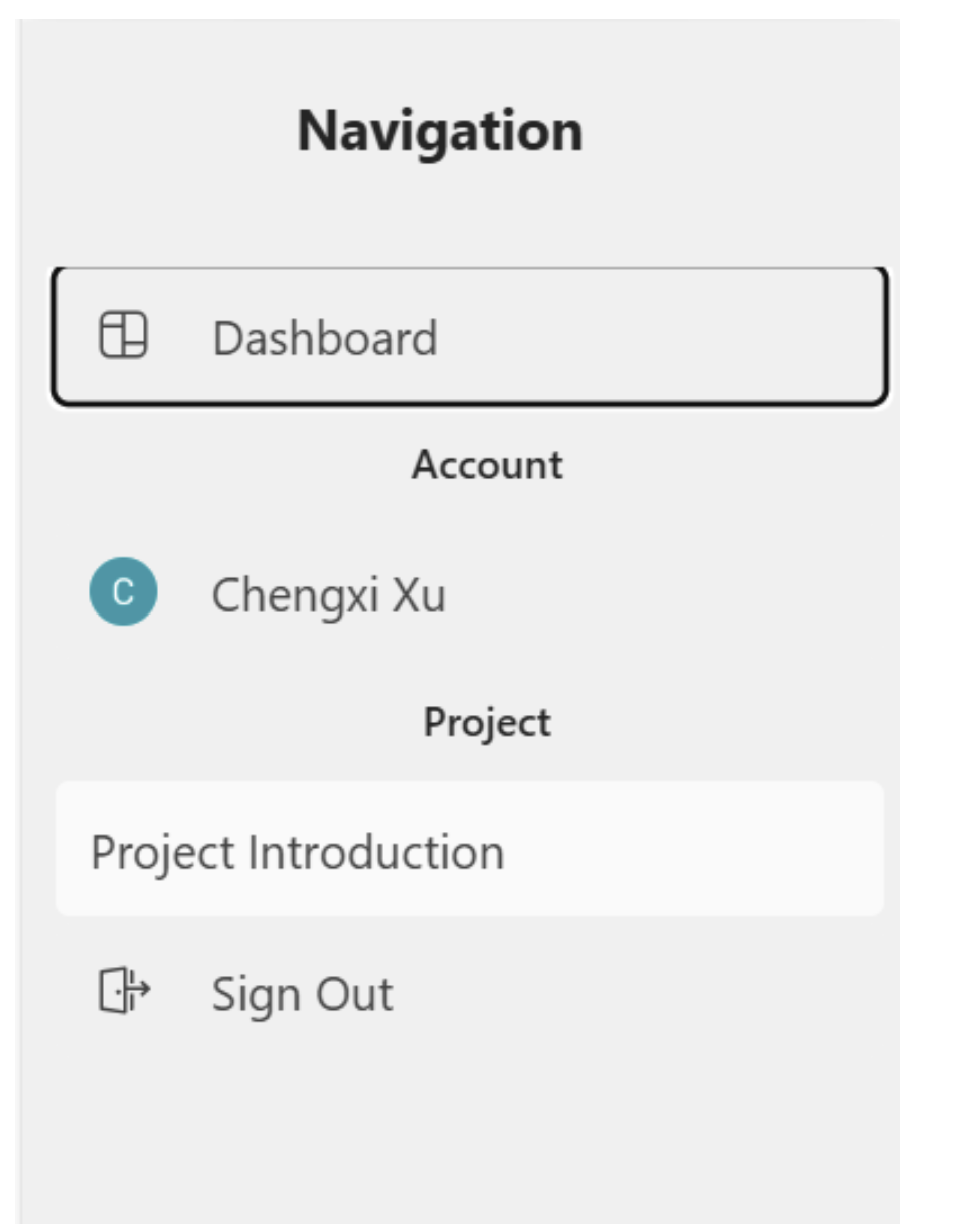
\includegraphics[height=1.0\textheight,width=1.0\textwidth,keepaspectratio]{images/fishsense_enduser/webapp_navigation.png}
    \end{minipage}
    \hfill
    \begin{minipage}{0.75\textwidth}
        \centering
        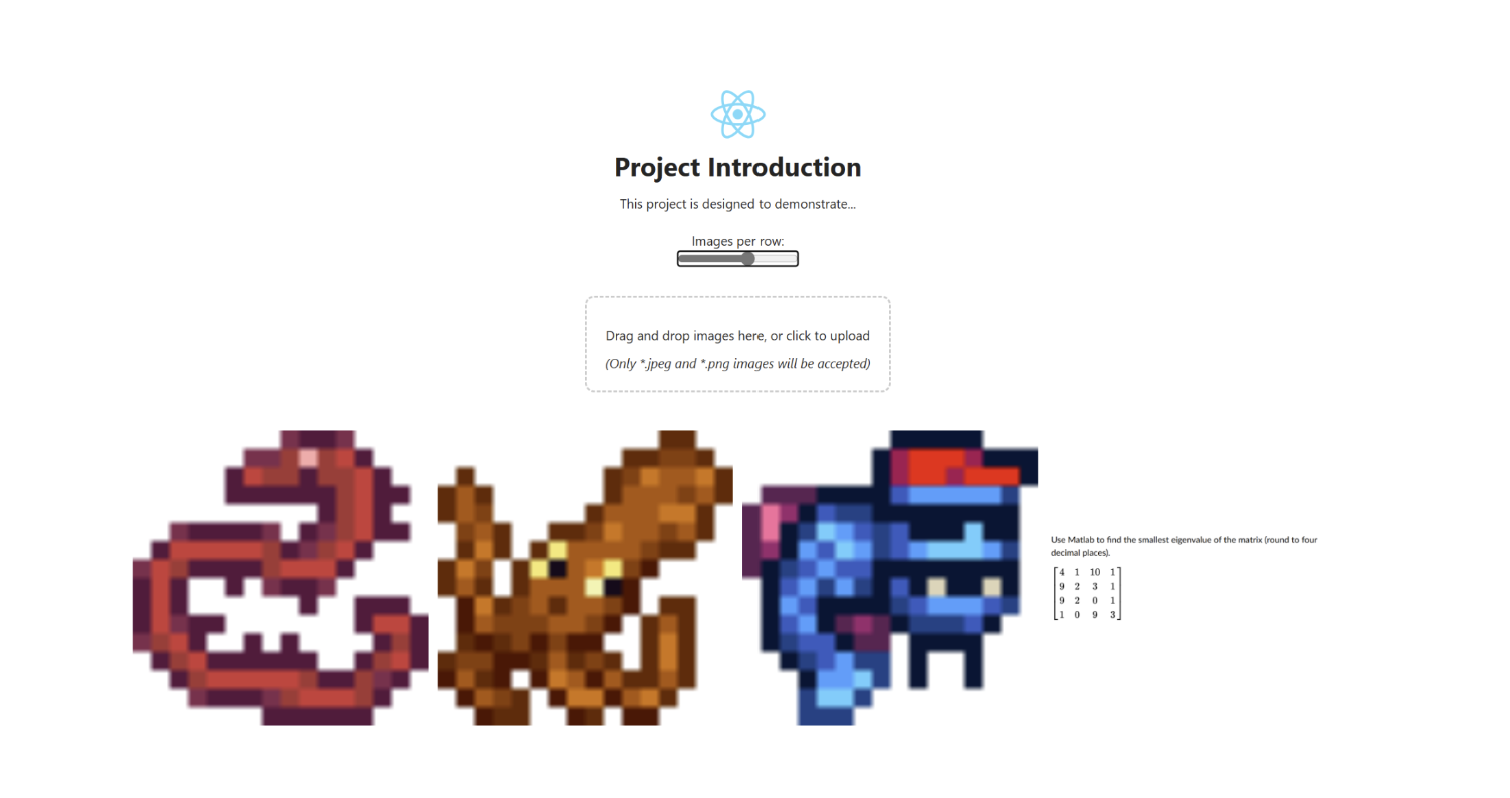
\includegraphics[width=\textwidth,keepaspectratio]{images/fishsense_enduser/webapp_gallery.png}
    \end{minipage}
\end{frame}


\begin{frame}{FishSense Web App: Front-End}
    \centering
    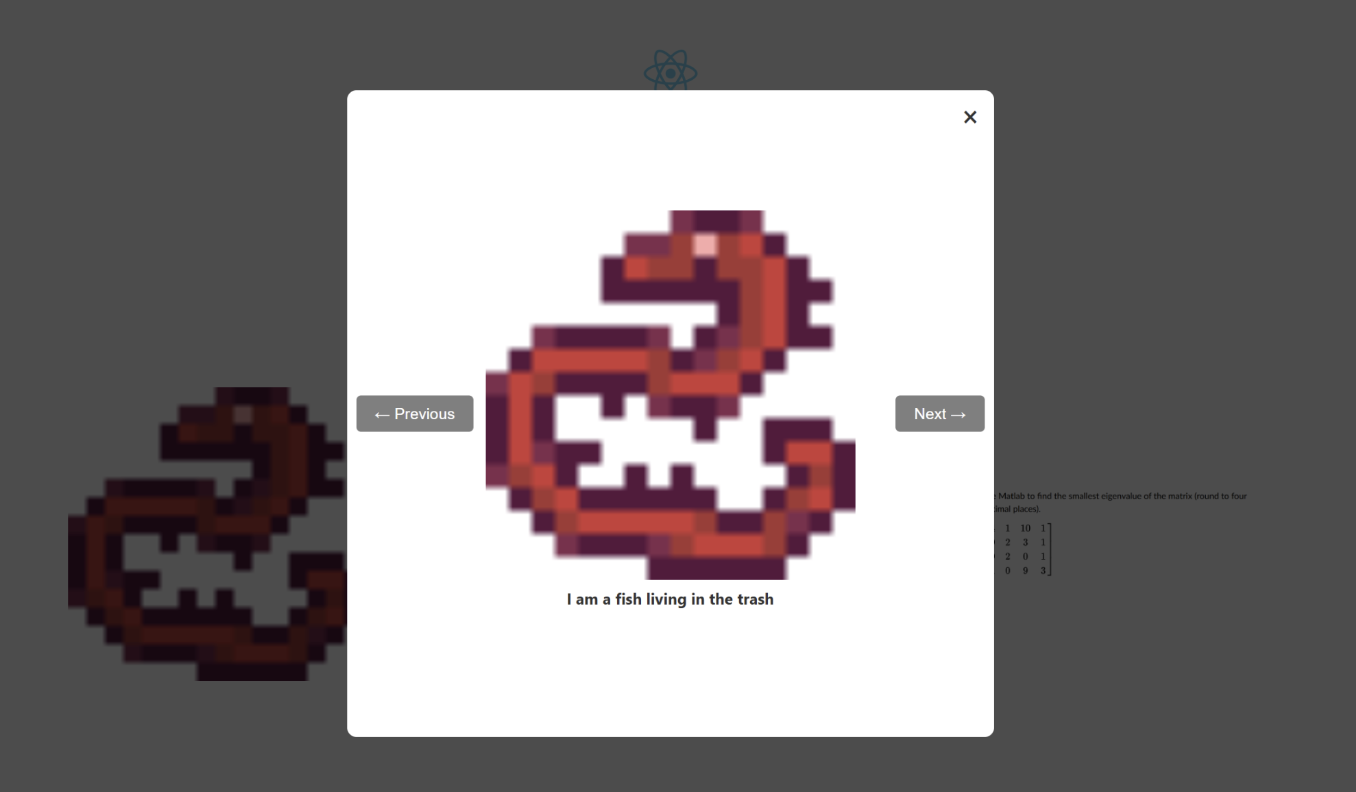
\includegraphics[height=0.8\textheight,width=0.8\textwidth,keepaspectratio]{images/fishsense_enduser/webapp_clickintoimage.png}
\end{frame}

% To create a slide with two columns, use the following:
% \begin{frame}{TITLE}
%     \begin{columns}
%         \begin{column}{0.5\textwidth}
%             COLUMN 1 BODY
%         \end{column}
%         \begin{column}{0.5\textwidth}
%             COLUMN 2 BODY
%         \end{column}
%     \end{columns}
% \end{frame}
